\section{Evaluation}
All experiments were run on Amazon EC2 using the p3.16xlarge instances.  Each instance has 8 Tesla V100 GPUs with 25Gbps Ethernet bandwidth. We conducted the following experiments:

\begin{enumerate}
    \item An end-to-end macrobenchmark measuring training throughput, for all three systems, utilizing up to 16 distinct instances (Figure~\ref{fig:sgd}).
    \item A microbenchmark that evaluates how how much of a bottleneck the datacenter network between nodes is (Figure~\ref{fig:infnet}).
    \item A microbenchmark that investigates the optimal number of GPUs per node. We find that using 8 GPUs per node yields worse scaling than using 4 GPUs per node, keeping the total number of GPUs constant (Figure~\ref{fig:8-vs-4-gpu}).
    \item A microbenchmark that investigates the best all-reduce strategy to use within a node (Figure~\ref{fig:intra-node-allreduce-strategy}).
\end{enumerate}

% \subsection{Single-Node Multi GPU SGD}
% Here we discuss some findings on Multi-GPU
% \subsection{Charts}

\subsection{End-to-end performance}
Figure~\ref{fig:sgd} shows the training throughput on ResNet-101 for three systems, Horovod, Distributed TensorFlow, and Ray.  In summary, our implementation in Ray is able to match Horovod and comes within 10\% of Distributed TensorFlow.  This result validates our hypothesis that the higher-level actor/task abstractions are able to match the SPMD/message-passing abstractions.

{\bf Weak Scaling.}  We note that the weak scaling factors, with 4 GPUs as baseline and with $2\times$ resource scaling at each step, are 1.9$\times$,1.9$\times$,3.7$\times$,7.3$\times$ for Horovod;
1.8$\times$,2.7$\times$,5.0$\times$,8.5$\times$ for Distributed TensorFlow;
and
1.8$\times$,2.2$\times$,4.1$\times$,7.3$\times$ for Ray.  Clearly, even the observed maximum 8.5$\times$ scaling  is far from ideal since $16\times$ as many GPUs are used; we surmise this is the exact reason that motivated several projects that investigate fast inter-GPUs interconnect, such as  NVIDIA's NVLink.

\begin{figure}[tb]
    \centering
    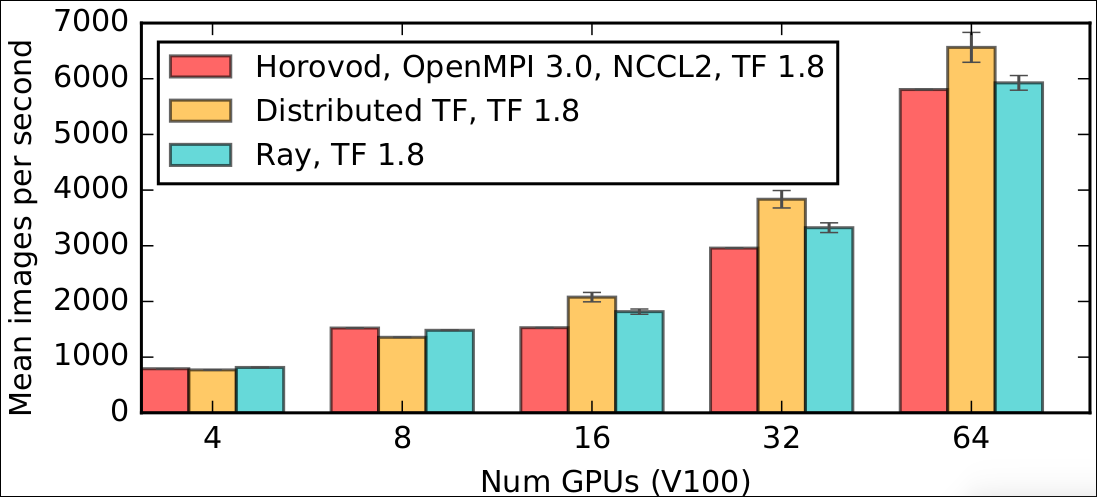
\includegraphics[width=5.1in,keepaspectratio]{fig/sgd.png}
    \caption{
    \small{
        Images per second reached when distributing the training of a
        ResNet-101 TensorFlow model (from the official TF benchmark).
        %The \System{} implementation matches the performance of Horovod and
        %is within 10\% of distributed TensorFlow.
        All experiments were run on p3.16xl instances connected by 25Gbps Ethernet, and
        workers allocated 4 GPUs per node as done in Horovod~\cite{horovod}.
        We note some measurement deviations from previously reported, likely
        due to hardware differences and
        recent TensorFlow performance improvements. We used
        OpenMPI 3.0, TF 1.8, and NCCL2 for all runs.
    }
    }
    \label{fig:sgd}
\end{figure}

\subsection{Inter-node allreduce}
To determine how much of a bottleneck the 25Gbps TCP network between nodes is, we run an experiment where all network transfers are replaced by 1-byte "noop" transfers and a sleep of the appropriate delay, thus emulating an idealized network operating at any speed we want it to. Figure \ref{fig:infnet} shows the performance of our SGD implementation with an emulated infinitely fast, 10Gbps, and 5Gbps network.

We find that our results with a 25Gbps network match the idealized 10Gbps network in practice. When using p3.8xl instances, which have a 10Gbps network, the throughput is slightly lower than estimated. This is likely due to inefficiences in the networking stack and the Ray object manager, which prevent full utilization of the network for small transfers.

\subsection{Intra-node allreduce}
Through our investigation we discovered two interesting scaling anomalies, as
shown in Figure~\ref{fig:8-vs-4-gpu}.

First, one of the compared systems, Horovod, yields a lower throughput when 16
GPUs (2 nodes) are used, compared to 8 GPUs (1 node).  This suggests that
Horovod's cross-machine communication overhead is so large that it dwarfs the
benefits of using twice as many processors.

Second, for our Ray implementation, using 8 GPUs per node (red bars) scales
noticeably worse than using 4 GPUs per node (blue bars), while fixing the total
number of GPUs fixed.  The former cases make use of less number of machines, so
cross-node communication should actually be faster than the latter cases.  We
believe that optimizing intra-node allreduce could lead to future performance improvements,
however it is non-trivial in practice due to intricate interactions with the TensorFlow
and CUDA schedulers.

\subsection{Intra-node Allreduce Strategies}
Figure~\ref{fig:intra-node-allreduce-strategy} compares two implementations of
allreduce within a node.  \emph{Simple} refers to designating one GPU as the
root, and have other local GPUs transfer gradients to it; afterwards the root
performs the reduce.  \emph{NCCL} refers to utilizing the NCCL library; under
the hood it's a set of hand-tuned CUDA kernels that occupy at least one
Streaming Multiprocessor.

The experiment shows that the Simple strategy outperforms NCCL when 4 GPUs per
node are used, and that the reverse holds true when 8 GPUs per node are
used. Both provide sublinear scaling. Based on analysis of Tensorflow timelines, 
we attribute the poor scalability of NCCL due to a bad interaction with the
Tensorflow scheduler that unnecessarily delays
the execution of downstream dependencies of NCCL ops.

% \begin{figure}[t]
%     \centering
%     % 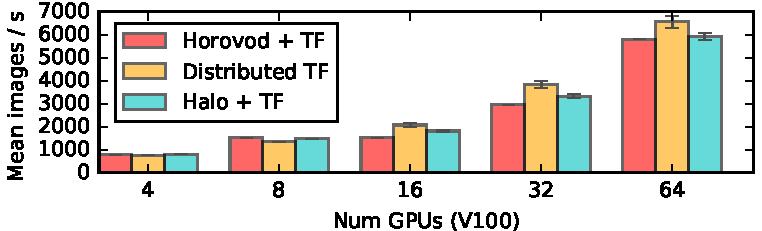
\includegraphics[width=3.1in,keepaspectratio]{fig/sgd_plot.pdf}
%     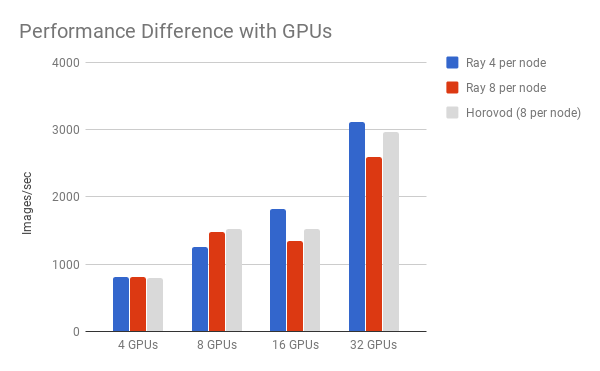
\includegraphics[width=3.1in,keepaspectratio]{fig/4to8.png}
%     \caption{
%     \small{
%         Performance differences for using 4 GPUs per node vs 8 GPUs per node. In all cases, we use the same hardware (p3.16xlarge). However, we see there are performance differences going from 4 GPUs to 8 GPUs when comparing the number of GPUs per node. We provide Horovod performance for reference.
%     }
%     }
%     \label{fig:8-vs-4-gpu}
% \end{figure}

% \begin{figure}[h]
%     \centering
%     % 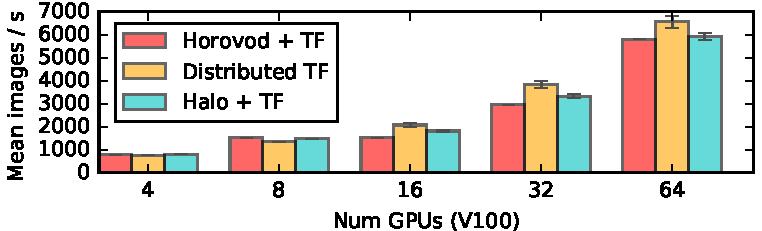
\includegraphics[width=3.1in,keepaspectratio]{fig/sgd_plot.pdf}
%     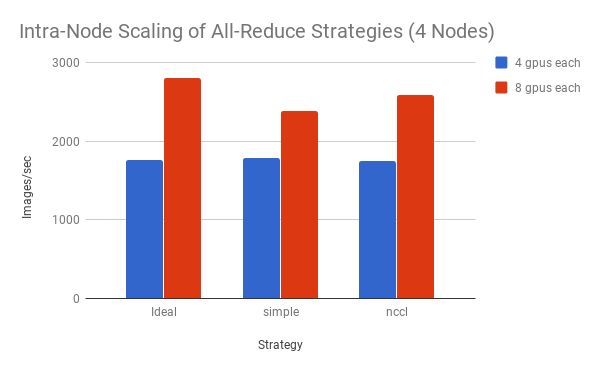
\includegraphics[width=3.1in,keepaspectratio]{fig/intranode.png}
%     \caption{ \small{ Changing the all reduce strategy among GPUs within a node,
%         and running a synchronous parameter server strategy between nodes. Ideal
%         is generated by taking the gradient of the a single GPU, bypassing any
%         communication overhead between GPUs on a single machine.  } }
%     % \caption{ \small{ Changing the all reduce strategy among GPUs within a node,
%     %     and running a synchronous parameter server strategy between nodes. Ideal
%     %     is generated by taking the gradient of the a single GPU, bypassing any
%     %     communication overhead between GPUs on a single machine. ``Simple''
%     %     performance simply takes an average across all of the GPUs {\color{red}
%     %       TODO: FIX THIS.}. ``NCCL'' performance uses the NCCL communication
%     %     primitives to perform an all-reduce across the GPUs. We see that even
%     %     though NCCL performance is better at 8 GPUs than ``Simple'', both
%     %     provide sublinear scaling when doubling the number of GPUs per machine.
%     %   } }

%     \label{fig:intra-node-allreduce-strategy}
% \end{figure}

\begin{figure}[tb]
    \centering
    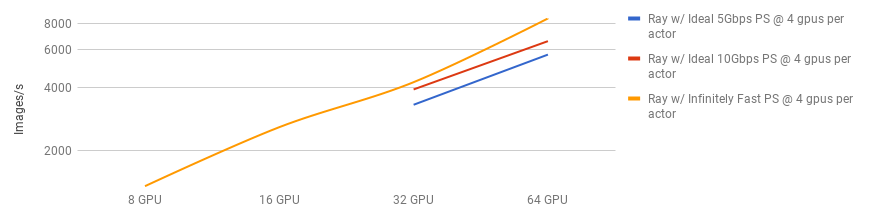
\includegraphics[width=5.1in,keepaspectratio]{fig/infnet.png}
    \caption{
    \small{
        Benchmarking our implementation with an infinitely fast emulated network (all transfers are truncated after 1-byte). This demonstrates that an idealized 10Gbps network is enough to match Horovod, and an infinitely fast network would be enough to beat both Horovod and Distributed TF by a significant fraction.
    }
    }
    \label{fig:infnet}
\end{figure}


\begin{figure}
\begin{subfigure}{0.45\textwidth}
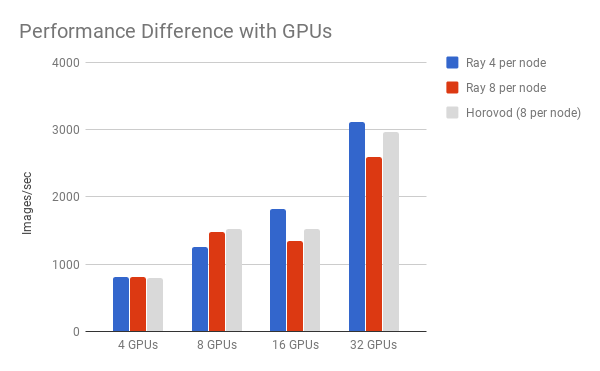
\includegraphics[width=1\textwidth]{fig/4to8.png}
% \caption{Sup}
    \caption{
    \small{
        Performance differences for using 4 GPUs per node vs 8 GPUs per node. In all cases, we use the same hardware (p3.16xlarge). However, we see there are performance differences going from 4 GPUs to 8 GPUs when comparing the number of GPUs per node. We provide Horovod performance for reference.
    }
    }
    \label{fig:8-vs-4-gpu}
\end{subfigure}\hspace{\fill}
\begin{subfigure}{0.45\textwidth}
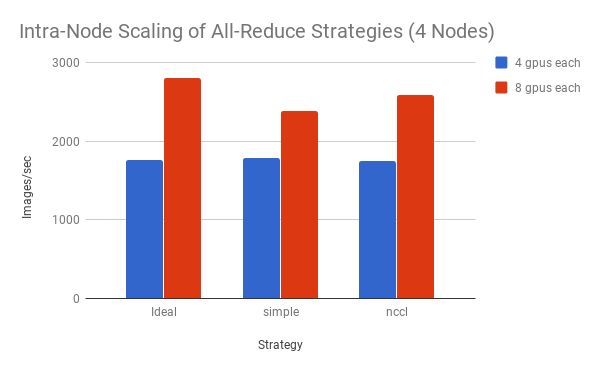
\includegraphics[width=1\textwidth]{fig/intranode.png}
% \caption{Inf}
    \caption{ \small{ Changing the all reduce strategy among GPUs within a node,
        and running a synchronous parameter server strategy between nodes. Ideal
        is generated by taking the gradient of the a single GPU, bypassing any
        communication overhead between GPUs on a single machine.  } }

    \label{fig:intra-node-allreduce-strategy}
\end{subfigure}
\caption{Microbenchmarks.}

\end{figure}
